\subsection{Sploty o dwóch mostach} % (fold)
\label{sub:twobridge}

Zajmiemy się teraz indeksem mostowym.
Wiemy, że węzeł trywialny jest jednomostowy.
Następne węzły (lub sploty) dwumostowe są pierwsze, alternujące, odwracalne i mają co najwyżej dwie składowe.

\begin{proposition}
\label{prp:two_bridge_tangle}
	Sploty z dwoma mostami to dokładnie sploty typu $D(T)$ dla pewnego supła wymiernego $T$.
\end{proposition}

Sploty otrzymane z supłów określa się czasami jako \emph{4-plats}.

\begin{proposition}
\label{prp:two_bridge_hyperbolic}
	Węzły dwumostowe, które nie są $(\pm 2, n)$-torusowymi, muszą być hiperbolicznymi.
\end{proposition}

\begin{proof}
	Podręcznik \cite{murasugi96} Murasugiego, twierdzenie 9.3.3 na stronie 138.
\end{proof}

%\todo[inline]{Murasugi Theorem 9.3.3 (138) lub Janiak-Osajca, Pogoda (34).}
% Aus der unten stehenden Klassifikation ergibt sich, dass man jede Verschlingung mit 2 Brücken wie im Bild rechts darstellen kann, wobei {\displaystyle a_{i}\in \mathbb {Z} } a_{i}\in \mathbb{Z }  die Anzahl der Halbtwists in der jeweiligen Box bezeichnet und für gerade bzw. ungerade {\displaystyle i} i positive {\displaystyle a_{i}} a_{i} links- bzw. rechtshändigen Halbtwists entsprechen.
% Diese Darstellung wird als Conway-Normalform bezeichnet.
% Man kann stets erreichen, dass alle {\displaystyle a_{i}} a_{i} dasselbe Vorzeichen haben.[1] Insbesondere gibt die Conway-Normalform dann ein alternierendes Knotendiagramm.[2]
%Insbesondere ist ein 2-Brücken-Knoten genau dann amphichiral, wenn {\displaystyle q^{2}\equiv -1\ mod\ p} q^{2}\equiv -1\ mod\ p ist.

Każdy splot dwumostowy można przedstawić następującym diagramem:
\begin{comment}
\[
    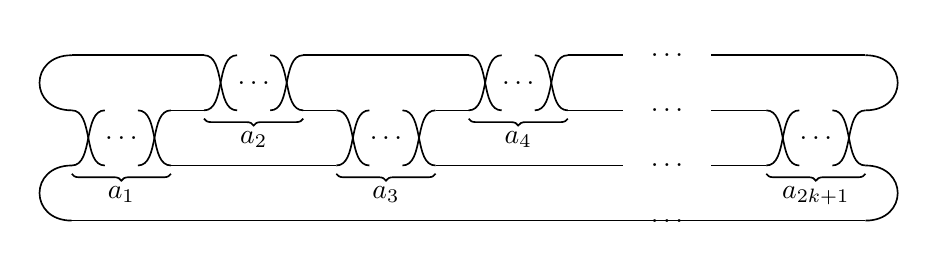
\begin{tikzpicture}[baseline=-0.65ex, xscale=0.14, yscale=0.07]
    \useasboundingbox (-40, -20) rectangle (40, 20);
        %%% A1
        \draw[semithick] (-36, -5) .. controls (-34,-5) and (-35, 5) .. (-33, 5);
        \draw[semithick] (-36,  5) .. controls (-34, 5) and (-35,-5) .. (-33,-5);
        \node at (-31.5, 0) {$\ldots$};
        \draw[semithick] (-30, -5) .. controls (-28,-5) and (-29, 5) .. (-27, 5);
        \draw[semithick] (-30,  5) .. controls (-28, 5) and (-29,-5) .. (-27,-5);
        %%% A2
        \draw[semithick] (-24,  5) .. controls (-22,  5) and (-23, 15) .. (-21, 15);
        \draw[semithick] (-24, 15) .. controls (-22, 15) and (-23,  5) .. (-21,  5);
        \node at (-19.5, 10) {$\ldots$};
        \draw[semithick] (-18,   5) .. controls (-16,  5) and (-17, 15) .. (-15, 15);
        \draw[semithick] (-18,  15) .. controls (-16, 15) and (-17,  5) .. (-15,  5);
        %%% A3
        \draw[semithick] (-12, -5) .. controls (-10,-5) and (-11, 5) .. (-9, 5);
        \draw[semithick] (-12,  5) .. controls (-10, 5) and (-11,-5) .. (-9,-5);
        \node at (-7.5, 0) {$\ldots$};
        \draw[semithick] (-6, -5) .. controls (-4,-5) and (-5, 5) .. (-3, 5);
        \draw[semithick] (-6,  5) .. controls (-4, 5) and (-5,-5) .. (-3,-5);
        %%% A4
        \draw[semithick] (0,  5) .. controls (2,  5) and (1, 15) .. (3, 15);
        \draw[semithick] (0, 15) .. controls (2, 15) and (1,  5) .. (3,  5);
        \node at (4.5, 10) {$\ldots$};
        \draw[semithick] (6,   5) .. controls (8,  5) and (7, 15) .. (9, 15);
        \draw[semithick] (6,  15) .. controls (8, 15) and (7,  5) .. (9,  5);
        %%% A 2k+1
        \draw[semithick] (27,  -5) .. controls (29,  -5) and (28, 5) .. (30, 5);
        \draw[semithick] (27, 5) .. controls (29, 5) and (28,  -5) .. (30,  -5);
        \node at (31.5, 0) {$\ldots$};
        \draw[semithick] (33,   -5) .. controls (35,  -5) and (34, 5) .. (36, 5);
        \draw[semithick] (33,  5) .. controls (35, 5) and (34,  -5) .. (36,  -5);
        %%%    - A3
        \draw[semithick] (-36, 15) to (-24, 15);
        %%% A1 - A3
        \draw[semithick] (-27, -5) to (-12, -5);
        %%% A1 - A2
        \draw[semithick] (-27,  5) to (-24,  5);
        %%% A2 - A3
        \draw[semithick] (-15,  5) to (-12,  5);
        %%% A2 - A4
        \draw[semithick] (-15, 15) to (0, 15);
        %%% A3 - A4
        \draw[semithick] (-3, 5) to (0, 5);
        %%%
        \draw[semithick] ( 9, 15) to (14, 15);
        \draw[semithick] ( 9,  5) to (14,  5);
        \draw[semithick] (-3, -5) to (14, -5);
        \node at (18,  15) {$\ldots$};
        \node at (18,   5) {$\ldots$};
        \node at (18,  -5) {$\ldots$};
        \node at (18, -15) {$\ldots$};
        \draw[semithick] (22, 15) to (36, 15);
        \draw[semithick] (22,  5) to (27,  5);
        \draw[semithick] (22, -5) to (27, -5);
        \draw[semithick] (-36, -15) to (36, -15);
        \draw[semithick] (-36, -15) [in=left,  out=left]  to (-36, -5);
        \draw[semithick] (-36,   5) [in=left,  out=left]  to (-36, 15);
        \draw[semithick] ( 36, -15) [in=right, out=right] to ( 36, -5);
        \draw[semithick] ( 36,   5) [in=right, out=right] to ( 36, 15);
        %
        \draw[semithick, decoration={brace,mirror,raise=3pt},decorate]  (-36, -5) -- node[below=4pt] {$a_1$}      (-27, -5);
        \draw[semithick, decoration={brace,mirror,raise=3pt},decorate]  (-24,  5) -- node[below=4pt] {$a_2$}      (-15,  5);
        \draw[semithick, decoration={brace,mirror,raise=3pt},decorate]  (-12, -5) -- node[below=4pt] {$a_3$}      ( -3, -5);
        \draw[semithick, decoration={brace,mirror,raise=3pt},decorate]  (  0,  5) -- node[below=4pt] {$a_4$}      (  9,  5);
        \draw[semithick, decoration={brace,mirror,raise=3pt},decorate]  ( 27, -5) -- node[below=4pt] {$a_{2k+1}$} ( 36, -5);
    \end{tikzpicture}
\]
\end{comment}


% \todo[inline]{Uwaga: Janiak-Osajca, Pogoda definiują osobny diagram o $2k$ skrętach!}

Oto reguła, zgodnie z którą wybieramy znaki liczb $a_i$:
jeśli $i$ jest nieparzyste, prawy skręt jest dodatni, jeśli parzyste -- lewy jest dodatni.
Przez analogię do supłów, definiujemy ułamek łańcuchowy
\[
	\frac \alpha \beta = a_1 + \frac{1}{a_2 + 1/\ldots}
\]

Wartość bezwzględna ułamka $\alpha/\beta$ zawsze przekracza $1$ i odwrotnie, każdy taki ułamek pochodzi od pewnego węzła.
Parę $(\alpha, \beta)$ (o względnie pierwszych współrzędnych) nazywamy typem węzła dwumostowego.

\begin{proposition}
\label{prp:tangle_equivalence}
	Dwumostowe sploty typów $(\alpha, \beta)$ oraz $(\alpha', \beta')$ są (pomijając orientację) równoważne wtedy i tylko wtedy, gdy $\alpha = \alpha'$ i $\beta \equiv \beta'$ lub $\beta \beta'\equiv 1$ modulo $\alpha$.
\end{proposition}

\begin{proof}
	Dowód opiera się na tym, że podwójnie cykliczna przestrzeń nakrywająca rozcięta wzdłuż splotu jest przestrzenią soczewkową typu $(\alpha, \beta)$.
	Nie definiowaliśmy nawet tych przestrzeni, szczegóły można znaleść w podręczniku \cite{murasugi96}.
\end{proof}

\begin{proposition}
\label{prp:chiral_tangles}
	Splot typu $(\alpha, \beta)$ jest achiralny dokładnie, gdy $\beta^2 \equiv -1 \mod \alpha$.
\end{proposition}


Węzłów dwumostowych nie można odróżniać od siebie samym wyznacznikiem, gdyż prawdziwe jest następujące stwierdzenie.

\begin{proposition}
\label{prp:tangle_determinant}
	Wyznacznikiem dwumostowego splotu typu $(\alpha, \beta)$ jest $\alpha$.
\end{proposition}

\begin{proof}
	Chcąc oszczędzić niektórym Czytelnikom cierpień odsyłamy po prostu do ,,Knoten mit zwei Brücken'' 1956 Schubert.
\end{proof}

\begin{proposition}
\label{prp:tangle_signature}
	Ropatrzmy węzeł dwumostowy typu $(\alpha, \beta)$, gdzie $0 < \beta < \alpha$ i $\beta$ jest nieparzyste.
	Niech $r_i$ będzie resztą z dzielenia $i\beta$ przez $2\alpha$ leżącą w przedziale $(-\alpha, \alpha)$ dla $i = 0, 1, \ldots, \alpha - 1$.
	Różnica między ilością dodatnich resz i ujemnych reszt to sygnatura węzła.
\end{proposition}

Wygląda na to, że jedynym niewyznaczonym do końca klasycznym niezmiennikiem jest liczba gordyjska.

% Koniec podsekcji Sploty o dwóch mostach
